\documentclass[xcolor=table,slidestop,compress,mathserif]{beamer}
\beamertemplatenavigationsymbolsempty
%\usepackage[no-math]{fontspec}
%\usepackage{xeCJK}
%\setCJKmainfont[BoldFont={Adobe Heiti Std}]{Adobe Song Std}
%\punctstyle{kaiming}
\usepackage{amssymb}
\usepackage{media9}
\usepackage{multimedia}
% setup tikz 
\usepackage{tikz}
\usetikzlibrary{shapes.geometric, arrows}
\tikzstyle{arrow} = [thick,->,>=stealth]
\tikzstyle{roundRec} = [rectangle, rounded corners, minimum width=1.5cm, minimum height=1cm,text centered, draw=black]
\tikzstyle{roundRecS} = [rectangle, rounded corners, minimum width=1.5cm, minimum height=0.5cm,text centered, draw=black]
\tikzstyle{rec} = [rectangle, minimum width=1.5cm, minimum height=1cm,text centered, draw=black]
\DeclareGraphicsExtensions{.pdf,.eps,.png,.jpg,.jpeg}
\graphicspath{{./figure/}}

\setbeamertemplate{items}[circle]
\usetheme{Warsaw}
\setbeamertemplate{headline}{}
\defbeamertemplate*{footline}{shadow theme}
{%
  \leavevmode%
  \hbox{\begin{beamercolorbox}[wd=.5\paperwidth,ht=2.5ex,dp=1.125ex,leftskip=.3cm
      plus1fil,rightskip=.3cm]{author in head/foot}%
    \usebeamerfont{author in
      head/foot}\insertshortinstitute\hfill\insertshortauthor
  \end{beamercolorbox}%
  \begin{beamercolorbox}[wd=.5\paperwidth,ht=2.5ex,dp=1.125ex,leftskip=.3cm,rightskip=.3cm
    plus1fil]{title in head/foot}%
    \usebeamerfont{title in
      head/foot}\hfill\insertframenumber\,/\,\inserttotalframenumber%
  \end{beamercolorbox}}%
  \vskip0pt%
}
\usepackage{graphicx}

\pgfdeclareimage[height=0.618cm]{logo}{figures/sjtulogoblue.png}
\logo{\pgfuseimage{logo}}

\def\hilite<#1>{%
  \temporal<#1>{\color{gray}}{\color{blue}}%
  {\color{blue!25}}}
% ------------------------------------------
\title{Audio Event Detection for \\ Automatic Scene Recognition}
\author{Xun Xu}
\institute[CS SJTU]{Department of Computer Science and Engineering \\ Shanghai
  Jiao Tong University}
\date{\today}
\begin{document}
\frame{\titlepage}

% show the outline 
\begin{frame}<beamer>[shrink=10]{Outline}
  \tableofcontents[sectionstyle=show,subsectionstyle=hide]
\end{frame}

% show outline when switch sections
\AtBeginSection[]{
  \begin{frame}<trans|beamer>[shrink=25]{Outline}
    \tableofcontents[sectionstyle=show/shaded,subsectionstyle=show/show/hide]
  \end{frame}
}

% ------------------------------------------

\section{Introduction}
\subsection{Problem Description}
\begin{frame}
  \frametitle{Problem Description}
	In this project, our problem is to recognize a scene where an audio is recorded. \\ 
	
	%\sound[label=show1, inlinesound]{}{show.wav}
	%\hyperlinkmovie[start=0s]{show1}{\beamerbutton{Play Sound}} \\

	%waveform 
	\vspace{0.5cm}
	\begin{columns}[c]
		\begin{column}{0.5\textwidth}
			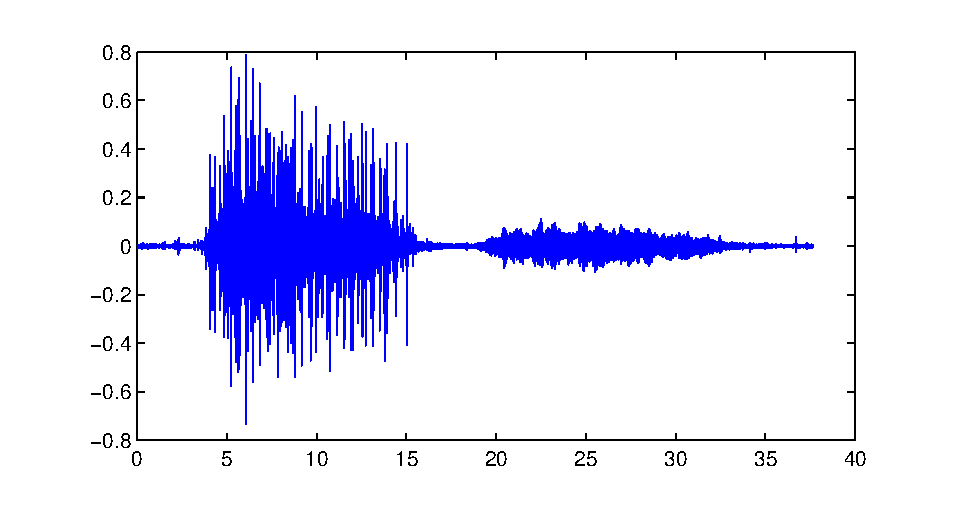
\includegraphics[scale=0.4]{./figure/tune_part.eps}
		\end{column}
		\begin{column}{0.05\textwidth}
			\centering
			$\Rightarrow$
		\end{column}
		\begin{column}{0.45\textwidth}
			\em{concert}
		\end{column}
	\end{columns}

\end{frame}
% ------------------------------------------
\subsection{Approach}
\begin{frame}
  \frametitle{Our Approach}
	Our approach is to detect the audible events in a clip. \\
	Then infer the scene from the detected events. 	
		
	\vspace{0.5cm}
	\begin{columns}[c]
		\begin{column}{0.5\textwidth}
			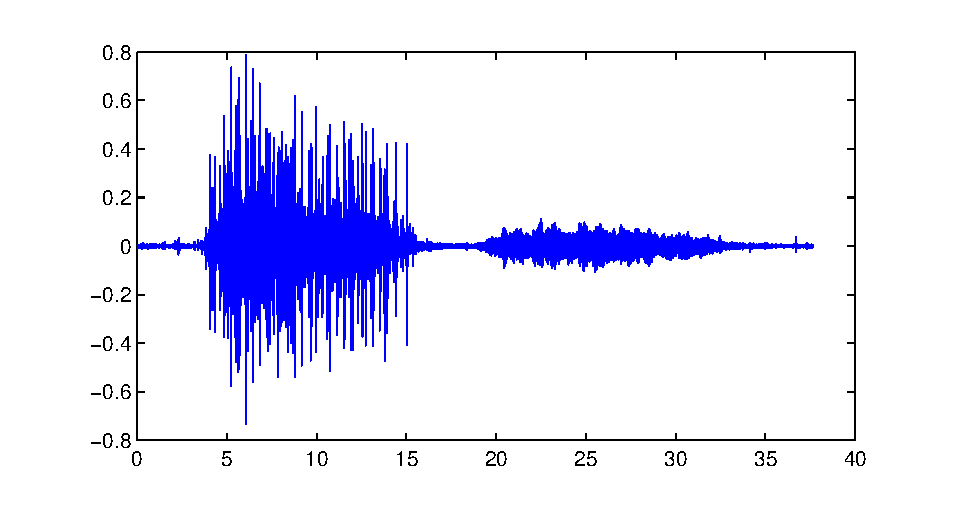
\includegraphics[scale=0.4]{./figure/tune_part.eps}
		\end{column}
		\begin{column}{0.05\textwidth}
			$\Rightarrow$
		\end{column}
		\begin{column}{0.2\textwidth}
			\em{applause, instrument}
		\end{column}
		\begin{column}{0.05\textwidth}
			$\Rightarrow$
		\end{column}
		\begin{column}{0.2\textwidth}
			\em{concert}
		\end{column}
	\end{columns}

\end{frame}
% ------------------------------------------
\begin{frame}
	\frametitle{Our Approach vs. Other Approaches}
	\begin{columns}[c]
		\begin{column}{0.5\textwidth}
			Our approach:\\ 
			\vspace{0.5cm}
			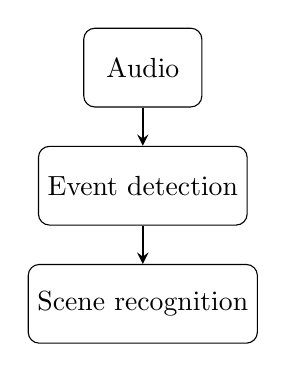
\begin{tikzpicture}[node distance=1.5cm]
				\node (audio) [roundRec] {Audio}; 
				\node (event) [roundRec, below of=audio] {Event detection}; 
				\node (scene) [roundRec, below of=event] {Scene recognition}; 
				\draw [arrow] (audio) -- (event);
				\draw [arrow] (event) -- (scene); 
			\end{tikzpicture}
		\end{column}
		\begin{column}{0.5\textwidth}
			Other approaches: \\ 
			\vspace{0.5cm}
			\begin{tikzpicture}[node distance=1.5cm]
				\node (audio) [roundRec] {Audio}; 
				\node (scene) [roundRec, below of=event] {Scene recognition}; 
				\draw [arrow] (audio) -- (scene);
			\end{tikzpicture}
		\end{column}
	\end{columns}

\end{frame}
% ------------------------------------------
\section{Audio Event Detection}
\subsection{Audible Event Taxonomy}
\begin{frame}
	\frametitle{Audible Event Taxonomy}	
	We labelled common audible events into 4 classes.\\
	There are 120 events in total. \\ 
	\vspace{0.5cm}
	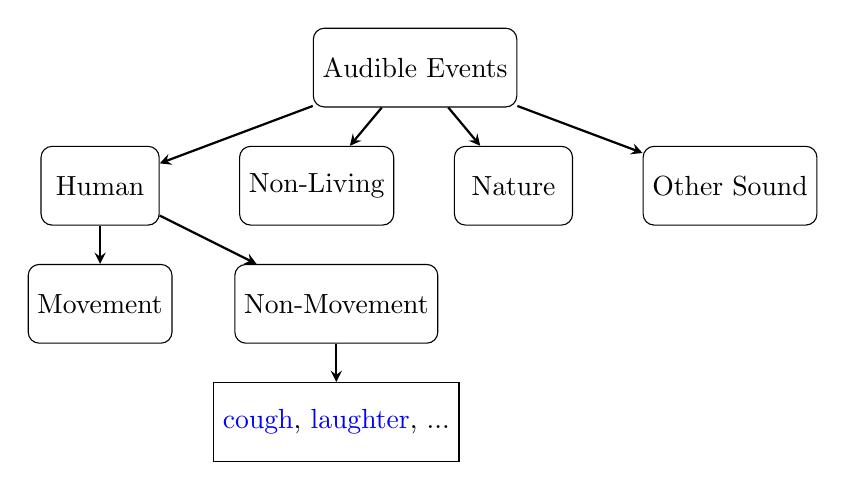
\begin{tikzpicture}[node distance=1.5cm]
		\node (event) [roundRec] {Audible Events}; 
		\node (human) [roundRec, below of=event, xshift=-4cm] {Human}; 
		\node (nonliving) [roundRec, below of=event, xshift=-1.25cm] {Non-Living}; 
		\node (nature) [roundRec, below of=event, xshift=1.25cm] {Nature}; 
		\node (other) [roundRec, below of=event, xshift=4cm] {Other Sound}; 
		\node (movement) [roundRec, below of=human] {Movement}; 
		\node (nonmovement) [roundRec, below of=human, xshift=3cm] {Non-Movement}; 
		\node (events) [rec, below of=nonmovement] {\textcolor{blue}{cough}, \textcolor{blue}{laughter}, ...}; 
		\draw [arrow] (event) -- (human);
		\draw [arrow] (event) -- (nonliving);
		\draw [arrow] (event) -- (nature);
		\draw [arrow] (event) -- (other); 
		\draw [arrow] (human) -- (movement); 
		\draw [arrow] (human) -- (nonmovement); 
		\draw [arrow] (nonmovement) -- (events); 
	\end{tikzpicture}
\end{frame}
% ------------------------------------------
\subsection{Audio Data}
\begin{frame}
  \frametitle{Audio Data}	
	We download the audio data for events from \\ Sound Search Engines (SSEs). \\ 
	For example, when we query ``cough'' in SSE: \\ 
	\begin{figure}
	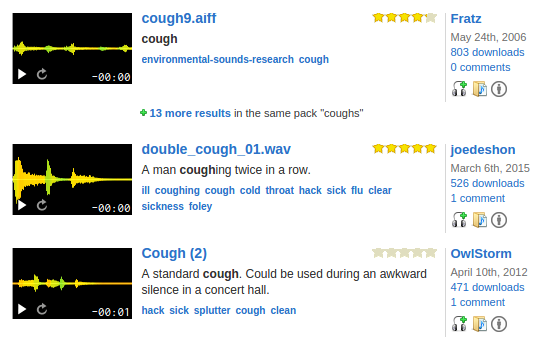
\includegraphics[scale=0.35]{figure/cough.png}
	\end{figure}
	We download clips from 1 second to 60 seconds. 
\end{frame}
% ------------------------------------------
\subsection{Preprocess and Feature Extraction}
\begin{frame}
	\frametitle{Preprocess and Feature Extraction}
	We first use Minimum Statistics to calculate the noise spectrum and subtract it from the input signal. \\ 
	Then we extract Mel-Frequency Cepstral Coefficients (MFCCs) from denoised signal.\\  
	\pause 
	% flowchart of mfcc 
	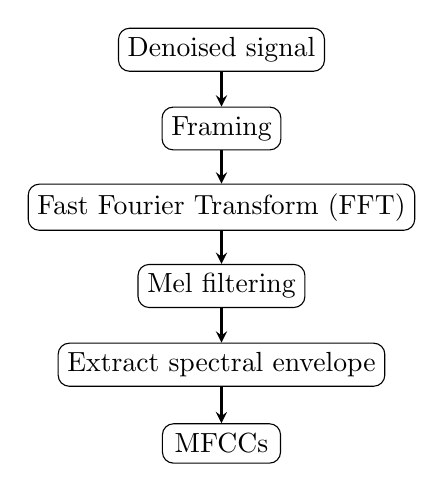
\begin{tikzpicture}[node distance=1cm]
		\node (audio) [roundRecS] {Denoised signal}; 
		\node (frame) [roundRecS, below of=audio] {Framing}; 
		\node (fft) [roundRecS, below of=frame] {Fast Fourier Transform (FFT)}; 
		\node (mel) [roundRecS, below of=fft] {Mel filtering}; 
		\node (envelope) [roundRecS, below of=mel] {Extract spectral envelope}; 
		\node (mfcc) [roundRecS, below of=envelope] {MFCCs}; 
		\draw [arrow] (audio) -- (frame);
		\draw [arrow] (frame) -- (fft); 
		\draw [arrow] (fft) -- (mel); 
		\draw [arrow] (mel) -- (envelope); 
		\draw [arrow] (envelope) -- (mfcc); 
	\end{tikzpicture}
	
\end{frame}
% ------------------------------------------
\subsection{Event Model}
\begin{frame}
	\frametitle{Event Model}	
	We use features to train Gaussian Mixture Models (GMMs). \\ 
	The training is done by Expectation-Maximization (EM) algorithm. \\  
	\begin{figure}
		%\resizebox{0.8\totalheight}{!}{% GNUPLOT: LaTeX picture with Postscript
\begingroup
  \makeatletter
  \providecommand\color[2][]{%
    \GenericError{(gnuplot) \space\space\space\@spaces}{%
      Package color not loaded in conjunction with
      terminal option `colourtext'%
    }{See the gnuplot documentation for explanation.%
    }{Either use 'blacktext' in gnuplot or load the package
      color.sty in LaTeX.}%
    \renewcommand\color[2][]{}%
  }%
  \providecommand\includegraphics[2][]{%
    \GenericError{(gnuplot) \space\space\space\@spaces}{%
      Package graphicx or graphics not loaded%
    }{See the gnuplot documentation for explanation.%
    }{The gnuplot epslatex terminal needs graphicx.sty or graphics.sty.}%
    \renewcommand\includegraphics[2][]{}%
  }%
  \providecommand\rotatebox[2]{#2}%
  \@ifundefined{ifGPcolor}{%
    \newif\ifGPcolor
    \GPcolorfalse
  }{}%
  \@ifundefined{ifGPblacktext}{%
    \newif\ifGPblacktext
    \GPblacktexttrue
  }{}%
  % define a \g@addto@macro without @ in the name:
  \let\gplgaddtomacro\g@addto@macro
  % define empty templates for all commands taking text:
  \gdef\gplbacktext{}%
  \gdef\gplfronttext{}%
  \makeatother
  \ifGPblacktext
    % no textcolor at all
    \def\colorrgb#1{}%
    \def\colorgray#1{}%
  \else
    % gray or color?
    \ifGPcolor
      \def\colorrgb#1{\color[rgb]{#1}}%
      \def\colorgray#1{\color[gray]{#1}}%
      \expandafter\def\csname LTw\endcsname{\color{white}}%
      \expandafter\def\csname LTb\endcsname{\color{black}}%
      \expandafter\def\csname LTa\endcsname{\color{black}}%
      \expandafter\def\csname LT0\endcsname{\color[rgb]{1,0,0}}%
      \expandafter\def\csname LT1\endcsname{\color[rgb]{0,1,0}}%
      \expandafter\def\csname LT2\endcsname{\color[rgb]{0,0,1}}%
      \expandafter\def\csname LT3\endcsname{\color[rgb]{1,0,1}}%
      \expandafter\def\csname LT4\endcsname{\color[rgb]{0,1,1}}%
      \expandafter\def\csname LT5\endcsname{\color[rgb]{1,1,0}}%
      \expandafter\def\csname LT6\endcsname{\color[rgb]{0,0,0}}%
      \expandafter\def\csname LT7\endcsname{\color[rgb]{1,0.3,0}}%
      \expandafter\def\csname LT8\endcsname{\color[rgb]{0.5,0.5,0.5}}%
    \else
      % gray
      \def\colorrgb#1{\color{black}}%
      \def\colorgray#1{\color[gray]{#1}}%
      \expandafter\def\csname LTw\endcsname{\color{white}}%
      \expandafter\def\csname LTb\endcsname{\color{black}}%
      \expandafter\def\csname LTa\endcsname{\color{black}}%
      \expandafter\def\csname LT0\endcsname{\color{black}}%
      \expandafter\def\csname LT1\endcsname{\color{black}}%
      \expandafter\def\csname LT2\endcsname{\color{black}}%
      \expandafter\def\csname LT3\endcsname{\color{black}}%
      \expandafter\def\csname LT4\endcsname{\color{black}}%
      \expandafter\def\csname LT5\endcsname{\color{black}}%
      \expandafter\def\csname LT6\endcsname{\color{black}}%
      \expandafter\def\csname LT7\endcsname{\color{black}}%
      \expandafter\def\csname LT8\endcsname{\color{black}}%
    \fi
  \fi
  \setlength{\unitlength}{0.0500bp}%
  \begin{picture}(7200.00,5040.00)%
    \gplgaddtomacro\gplbacktext{%
      \csname LTb\endcsname%
      \put(726,440){\makebox(0,0)[r]{\strut{} 0}}%
      \put(726,1018){\makebox(0,0)[r]{\strut{} 0.2}}%
      \put(726,1596){\makebox(0,0)[r]{\strut{} 0.4}}%
      \put(726,2174){\makebox(0,0)[r]{\strut{} 0.6}}%
      \put(726,2752){\makebox(0,0)[r]{\strut{} 0.8}}%
      \put(726,3330){\makebox(0,0)[r]{\strut{} 1}}%
      \put(726,3908){\makebox(0,0)[r]{\strut{} 1.2}}%
      \put(726,4486){\makebox(0,0)[r]{\strut{} 1.4}}%
      \put(1453,220){\makebox(0,0){\strut{}-4}}%
      \put(2642,220){\makebox(0,0){\strut{}-2}}%
      \put(3831,220){\makebox(0,0){\strut{} 0}}%
      \put(5020,220){\makebox(0,0){\strut{} 2}}%
      \put(6209,220){\makebox(0,0){\strut{} 4}}%
    }%
    \gplgaddtomacro\gplfronttext{%
      \csname LTb\endcsname%
      \put(2407,4602){\makebox(0,0){\strut{}Gaussian Distribution}}%
      \csname LTb\endcsname%
      \put(1449,4382){\makebox(0,0)[l]{\strut{}$\mu$ =  0.5 $\sigma$ = 0.5}}%
      \csname LTb\endcsname%
      \put(1449,4162){\makebox(0,0)[l]{\strut{}$\mu$ =  2.0 $\sigma$ = 1.0}}%
      \csname LTb\endcsname%
      \put(1449,3942){\makebox(0,0)[l]{\strut{}$\mu$ = -1.0 $\sigma$ = 2.0}}%
      \csname LTb\endcsname%
      \put(1449,3722){\makebox(0,0)[l]{\strut{}GMM}}%
    }%
    \gplbacktext
    \put(0,0){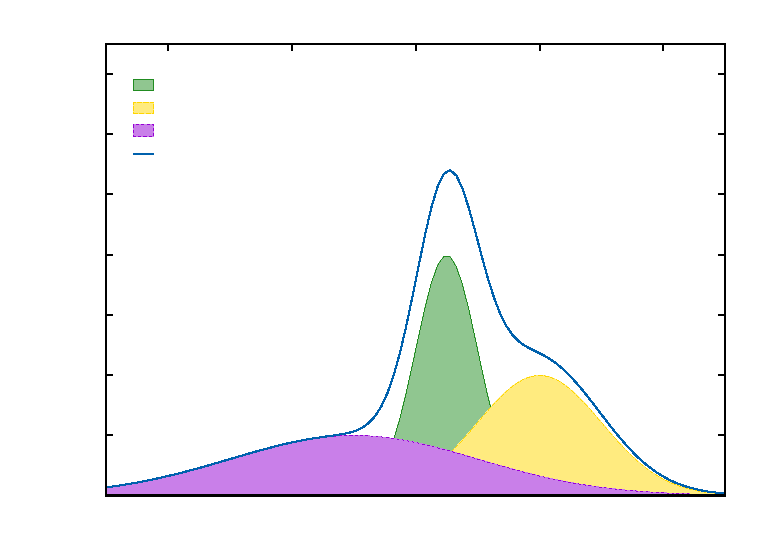
\includegraphics{gmm}}%
    \gplfronttext
  \end{picture}%
\endgroup
}
		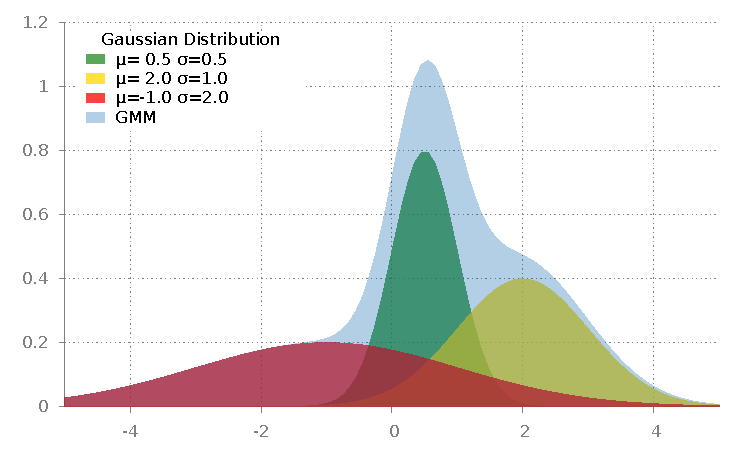
\includegraphics[scale=0.6]{figure/gmm.pdf}
		\caption{A GMM with three components}
	\end{figure}
\end{frame}
% ------------------------------------------
\section{Scene Recognition}
\subsection{Scene Extraction}
\begin{frame}
	\frametitle{Scene Extraction}	
	We use the scripts for movies, plays and TV series to extract the scenes. \\ 
	Below is a script example. 
	We call it a \textit{context}, including a scene, and some descriptive sentences. 
	\begin{table}[h]
		\begin{tabular}{|l|}
		\hline
		INT. LEONARD'S \textcolor{red}{BATHROOM} - Night \\ 
		Leonard turns on the light, revealing a shower, toilet and sink.\\
		He removes toiletries from the grocery bag and places them inside. \\ 
		\hline
		\end{tabular}
	\end{table}
\end{frame}
% ------------------------------------------
\begin{frame}
	\frametitle{Scene Extraction}
	We use Natural Language Process (NLP) tools to process a context, and eliminate the following type of words: \\ 
	\begin{itemize}
		\item{Person names} 
		\item{Time indicator}
		\item{Location names}
		\item{Adjective, determiner, number, ...}
	\end{itemize}

	\begin{table}[htb]
	\centering
	\caption{Top 10 Occurred Scenes}
	\resizebox{0.3\textwidth}{!}{
		\begin{tabular}{ll}
		\hline
		Scene & Occurrence \\
		\hline
		house & 3537 \\ 
		office & 3259 \\ 
		apartment & 2919 \\ 
		room & 2580 \\ 
		bedroom & 2257 \\ 
		car & 1699 \\ 
		street & 1622 \\ 
		kitchen & 1431 \\ 
		living room & 1374 \\ 
		tardis & 1259 \\ 
		\hline
		\end{tabular}
	}
	\end{table}
\end{frame}
% ------------------------------------------
\subsection{Scene-Event Relation Mining}
\begin{frame}
	\frametitle{Scene-Event Relation Mining}
	To get the relation between scenes and audible events, \\ 
	we match the context in a script with our predefined audible events. \\ 
	\begin{table}[h]
		\begin{tabular}{|l|}
		\hline
		INT. LEONARD'S \textcolor{red}{BATHROOM} - Night \\ 
		Leonard turns on the light, revealing a \textcolor{blue}{shower}, \textcolor{blue}{toilet} and \textcolor{blue}{sink}.\\
		He removes toiletries from the grocery bag and places them inside. \\ 
		\hline
		\end{tabular}
	\end{table}
\end{frame}
% ------------------------------------------
\begin{frame}
	\frametitle{Scene-Event Relation Mining}
	Based on the idea of Term-Frequency-Inverse Document Frequency (TFIDF), we calculate two scores of an event $e$, to a scene $s$. 
	\begin{enumerate}
		\item{$TF=log(1+f(e,s))$}\\
		$f(e,s)$ is the number of contexts $e$ appears in all contexts under scene $s$. 
		\item{$IDF=1+log(\frac{N}{N_e})$} \\ 
		$N$ is the number of scenes. 
		$N_e$ is the number of scenes in which event $e$ appears. 
	\end{enumerate}
	These two scores are then multiplied, and used as the importance of an event to a scene. 		
	\begin{equation}
		TFIDF = TF \times IDF 
	\end{equation}	
\end{frame}
% ------------------------------------------
\begin{frame}
	\frametitle{Scene-Event Relation Mining}
	\begin{table}[htb!]
	\caption{An example of scene-event map}
	\resizebox{1\textwidth}{!}{
	\begin{tabular}{ll}
	\hline
	Scene     & Top 10 events ranked by TF-IDf\\
	\hline
	bathroom & running+water, toilet, faucet, toothbrush, shower, drawer, drain, talk, paper, bowl \\ 
	beach & seagull, sand, boat, talk, wave, sea, car, laughter, drink, wood, running \\ 
	concert & piano, applause, crowd, chorus, child, cry, talk \\ 
	forest & tree, wood, dirt, talk, running, bird, river, car, leaf, grass, wind\\ 
	kitchen & drawer, cutlery, microwave, dish, kettle, talk, bowl, phone, toaster, running+water\\ 
	office & desk, drawer, page+turn, talk, phone, printer, paper, chair, leaf, typewriter\\
	park & talk, car, tree, laughter, dog, child, grass, crowd, running, phone\\ 
	restaurant & talk, drink, laughter, phone, car, leaf, paper, dish, ring, chair, write \\ 
	street & car, truck, subway, talk, traffic, engine, siren, phone, running, laughter \\ 
	subway station & subway, train, car, tube, talk, pace, crowd, metal, phone, vehicle \\ 
	\hline
	\end{tabular}
	}
	\end{table}
\end{frame}
% ------------------------------------------
\subsection{Audio Segmentation}
\begin{frame}
	\frametitle{Audio Segmentation}	
	In testing, we segment the audio into smaller parts for event detection. 
	We set two thresholds based on the following two features: 
	\begin{enumerate}
		\item{Frame Energy} \\ 
		The averaged energy of a frame, calculated as: 
		\begin{equation}
		E_i = \frac{\sum\limits_{n=1}^N(x_i(n))}{N}
		\end{equation}
		\item{Spectral Centroid} \\ 
		The ``center'' of frequency, calculated as: 
		\begin{equation}
		C_i = \frac{\sum\limits_{k=1}^Nk\times Amp(k)}{\sum\limits_{k=1}^NAmp(k)}
		\end{equation}
	\end{enumerate}
\end{frame}
% ------------------------------------------
\begin{frame}
	\frametitle{Audio Segmentation}
	\begin{figure}
	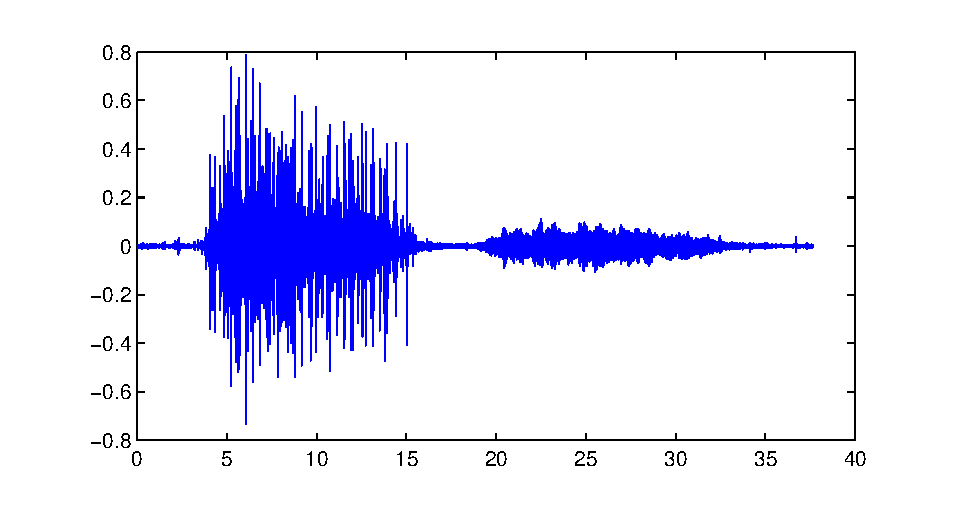
\includegraphics[scale=0.5]{figure/tune_part.eps}
	\caption{A example audio clip}
	\end{figure}
\end{frame}
% ------------------------------------------
\begin{frame}
	\frametitle{Audio Segmentation}
	
	\begin{figure}[htb]
	\centering
	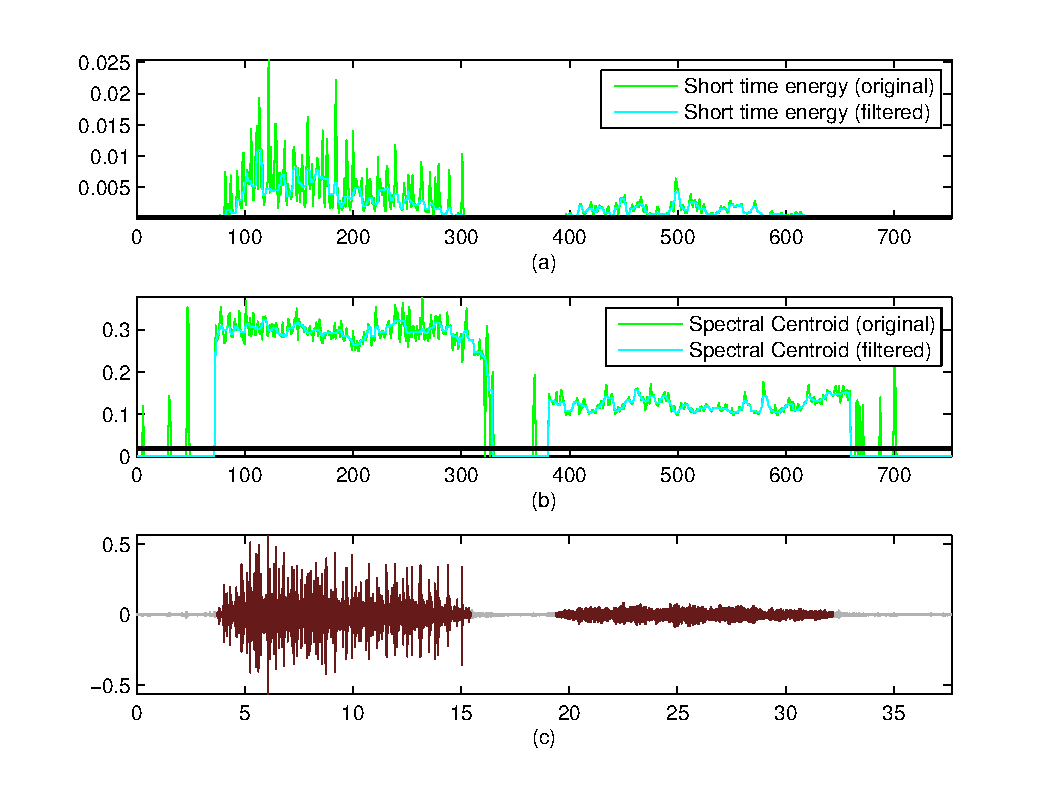
\includegraphics[scale=0.5]{figure/segment.pdf}
	\caption{A segmentation example}
	\label{fig:segment}
	\end{figure}
\end{frame}
% ------------------------------------------
\subsection{Scene Inference}
\begin{frame}
	\frametitle{Scene Inference}	
	For each segment, we evaluate it with our trained GMMs. \\ 
	We choose the top three detected events for scene voting. \\ 
	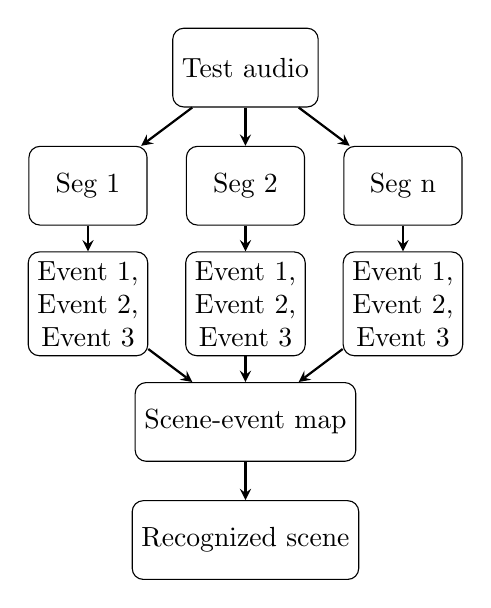
\begin{tikzpicture}[node distance=1.5cm, every text node part/.style={align=center}]
		\centering
		\node (audio) [roundRec] {Test audio}; 
		\node (seg1) [roundRec, below of=audio, xshift=-2cm] {Seg 1}; 
		\node (seg2) [roundRec, below of=audio] {Seg 2}; 
		\node (segn) [roundRec, below of=audio, xshift=2cm] {Seg n}; 
		\node (event1) [roundRec, below of=seg1] {Event 1, \\ Event 2, \\ Event 3}; 
		\node (event2) [roundRec, below of=seg2] {Event 1, \\ Event 2, \\ Event 3}; 
		\node (eventn) [roundRec, below of=segn] {Event 1, \\ Event 2, \\ Event 3}; 
		\node (map) [roundRec, below of=event2] {Scene-event map}; 	
		\node (scene) [roundRec, below of=map] {Recognized scene};
		\draw [arrow] (audio) -- (seg1);
		\draw [arrow] (audio) -- (seg2);
		\draw [arrow] (audio) -- (segn);
		\draw [arrow] (seg1) -- (event1); 
		\draw [arrow] (seg2) -- (event2); 
		\draw [arrow] (segn) -- (eventn); 
		\draw [arrow] (event1) -- (map); 
		\draw [arrow] (event2) -- (map); 
		\draw [arrow] (eventn) -- (map); 
		\draw [arrow] (map) -- (scene); 
	\end{tikzpicture}
\end{frame}
% ------------------------------------------
\section{Evaluation}
\subsection{Event Detection Evaluation}
\begin{frame}
	\frametitle{Component Number Evaluation}
	Gaussian Mixture Model distribution: \\ 
	\begin{equation}
	P(\mathbf{x}|\mathbf{\pi},\mathbf{\mu},\Sigma) = \sum_{k = 1}^{\textcolor{red}{M}} \pi_k
	\mathcal{N}(\mathbf{x}|\mathbf{\mu}_k, \Sigma_k),
	\end{equation} 

	\begin{figure}[htb!]
	\centering
	\resizebox{0.75\totalheight}{!}{% GNUPLOT: LaTeX picture with Postscript
\begingroup
  \makeatletter
  \providecommand\color[2][]{%
    \GenericError{(gnuplot) \space\space\space\@spaces}{%
      Package color not loaded in conjunction with
      terminal option `colourtext'%
    }{See the gnuplot documentation for explanation.%
    }{Either use 'blacktext' in gnuplot or load the package
      color.sty in LaTeX.}%
    \renewcommand\color[2][]{}%
  }%
  \providecommand\includegraphics[2][]{%
    \GenericError{(gnuplot) \space\space\space\@spaces}{%
      Package graphicx or graphics not loaded%
    }{See the gnuplot documentation for explanation.%
    }{The gnuplot epslatex terminal needs graphicx.sty or graphics.sty.}%
    \renewcommand\includegraphics[2][]{}%
  }%
  \providecommand\rotatebox[2]{#2}%
  \@ifundefined{ifGPcolor}{%
    \newif\ifGPcolor
    \GPcolorfalse
  }{}%
  \@ifundefined{ifGPblacktext}{%
    \newif\ifGPblacktext
    \GPblacktexttrue
  }{}%
  % define a \g@addto@macro without @ in the name:
  \let\gplgaddtomacro\g@addto@macro
  % define empty templates for all commands taking text:
  \gdef\gplbacktext{}%
  \gdef\gplfronttext{}%
  \makeatother
  \ifGPblacktext
    % no textcolor at all
    \def\colorrgb#1{}%
    \def\colorgray#1{}%
  \else
    % gray or color?
    \ifGPcolor
      \def\colorrgb#1{\color[rgb]{#1}}%
      \def\colorgray#1{\color[gray]{#1}}%
      \expandafter\def\csname LTw\endcsname{\color{white}}%
      \expandafter\def\csname LTb\endcsname{\color{black}}%
      \expandafter\def\csname LTa\endcsname{\color{black}}%
      \expandafter\def\csname LT0\endcsname{\color[rgb]{1,0,0}}%
      \expandafter\def\csname LT1\endcsname{\color[rgb]{0,1,0}}%
      \expandafter\def\csname LT2\endcsname{\color[rgb]{0,0,1}}%
      \expandafter\def\csname LT3\endcsname{\color[rgb]{1,0,1}}%
      \expandafter\def\csname LT4\endcsname{\color[rgb]{0,1,1}}%
      \expandafter\def\csname LT5\endcsname{\color[rgb]{1,1,0}}%
      \expandafter\def\csname LT6\endcsname{\color[rgb]{0,0,0}}%
      \expandafter\def\csname LT7\endcsname{\color[rgb]{1,0.3,0}}%
      \expandafter\def\csname LT8\endcsname{\color[rgb]{0.5,0.5,0.5}}%
    \else
      % gray
      \def\colorrgb#1{\color{black}}%
      \def\colorgray#1{\color[gray]{#1}}%
      \expandafter\def\csname LTw\endcsname{\color{white}}%
      \expandafter\def\csname LTb\endcsname{\color{black}}%
      \expandafter\def\csname LTa\endcsname{\color{black}}%
      \expandafter\def\csname LT0\endcsname{\color{black}}%
      \expandafter\def\csname LT1\endcsname{\color{black}}%
      \expandafter\def\csname LT2\endcsname{\color{black}}%
      \expandafter\def\csname LT3\endcsname{\color{black}}%
      \expandafter\def\csname LT4\endcsname{\color{black}}%
      \expandafter\def\csname LT5\endcsname{\color{black}}%
      \expandafter\def\csname LT6\endcsname{\color{black}}%
      \expandafter\def\csname LT7\endcsname{\color{black}}%
      \expandafter\def\csname LT8\endcsname{\color{black}}%
    \fi
  \fi
  \setlength{\unitlength}{0.0500bp}%
  \begin{picture}(7200.00,5040.00)%
    \gplgaddtomacro\gplbacktext{%
      \csname LTb\endcsname%
      \put(946,704){\makebox(0,0)[r]{\strut{} 0}}%
      \csname LTb\endcsname%
      \put(946,1383){\makebox(0,0)[r]{\strut{} 0.1}}%
      \csname LTb\endcsname%
      \put(946,2061){\makebox(0,0)[r]{\strut{} 0.2}}%
      \csname LTb\endcsname%
      \put(946,2740){\makebox(0,0)[r]{\strut{} 0.3}}%
      \csname LTb\endcsname%
      \put(946,3418){\makebox(0,0)[r]{\strut{} 0.4}}%
      \csname LTb\endcsname%
      \put(946,4097){\makebox(0,0)[r]{\strut{} 0.5}}%
      \csname LTb\endcsname%
      \put(946,4775){\makebox(0,0)[r]{\strut{} 0.6}}%
      \csname LTb\endcsname%
      \put(1078,484){\makebox(0,0){\strut{} 0}}%
      \csname LTb\endcsname%
      \put(1714,484){\makebox(0,0){\strut{} 5}}%
      \csname LTb\endcsname%
      \put(2350,484){\makebox(0,0){\strut{} 10}}%
      \csname LTb\endcsname%
      \put(2986,484){\makebox(0,0){\strut{} 15}}%
      \csname LTb\endcsname%
      \put(3622,484){\makebox(0,0){\strut{} 20}}%
      \csname LTb\endcsname%
      \put(4259,484){\makebox(0,0){\strut{} 25}}%
      \csname LTb\endcsname%
      \put(4895,484){\makebox(0,0){\strut{} 30}}%
      \csname LTb\endcsname%
      \put(5531,484){\makebox(0,0){\strut{} 35}}%
      \csname LTb\endcsname%
      \put(6167,484){\makebox(0,0){\strut{} 40}}%
      \csname LTb\endcsname%
      \put(6803,484){\makebox(0,0){\strut{} 45}}%
      \put(176,2739){\rotatebox{-270}{\makebox(0,0){\strut{}Average F-measure}}}%
      \put(3940,154){\makebox(0,0){\strut{}Component Number}}%
    }%
    \gplgaddtomacro\gplfronttext{%
    }%
    \gplbacktext
    \put(0,0){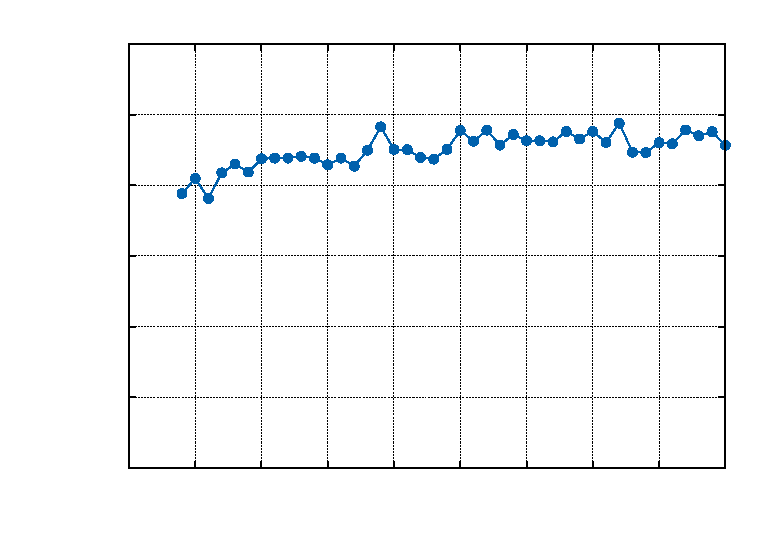
\includegraphics{component}}%
    \gplfronttext
  \end{picture}%
\endgroup
}
	\caption{F-measure for different component number}
	\label{fig:component}
	\end{figure}
\end{frame}
% ------------------------------------------
\begin{frame}
	\frametitle{Componnent Number Evaluation}
	After comparing F-measure and running time, we choose 18 as our component number. 
	\begin{figure}[htb!]
	\centering
	\resizebox{0.8\totalheight}{!}{% GNUPLOT: LaTeX picture with Postscript
\begingroup
  \makeatletter
  \providecommand\color[2][]{%
    \GenericError{(gnuplot) \space\space\space\@spaces}{%
      Package color not loaded in conjunction with
      terminal option `colourtext'%
    }{See the gnuplot documentation for explanation.%
    }{Either use 'blacktext' in gnuplot or load the package
      color.sty in LaTeX.}%
    \renewcommand\color[2][]{}%
  }%
  \providecommand\includegraphics[2][]{%
    \GenericError{(gnuplot) \space\space\space\@spaces}{%
      Package graphicx or graphics not loaded%
    }{See the gnuplot documentation for explanation.%
    }{The gnuplot epslatex terminal needs graphicx.sty or graphics.sty.}%
    \renewcommand\includegraphics[2][]{}%
  }%
  \providecommand\rotatebox[2]{#2}%
  \@ifundefined{ifGPcolor}{%
    \newif\ifGPcolor
    \GPcolorfalse
  }{}%
  \@ifundefined{ifGPblacktext}{%
    \newif\ifGPblacktext
    \GPblacktexttrue
  }{}%
  % define a \g@addto@macro without @ in the name:
  \let\gplgaddtomacro\g@addto@macro
  % define empty templates for all commands taking text:
  \gdef\gplbacktext{}%
  \gdef\gplfronttext{}%
  \makeatother
  \ifGPblacktext
    % no textcolor at all
    \def\colorrgb#1{}%
    \def\colorgray#1{}%
  \else
    % gray or color?
    \ifGPcolor
      \def\colorrgb#1{\color[rgb]{#1}}%
      \def\colorgray#1{\color[gray]{#1}}%
      \expandafter\def\csname LTw\endcsname{\color{white}}%
      \expandafter\def\csname LTb\endcsname{\color{black}}%
      \expandafter\def\csname LTa\endcsname{\color{black}}%
      \expandafter\def\csname LT0\endcsname{\color[rgb]{1,0,0}}%
      \expandafter\def\csname LT1\endcsname{\color[rgb]{0,1,0}}%
      \expandafter\def\csname LT2\endcsname{\color[rgb]{0,0,1}}%
      \expandafter\def\csname LT3\endcsname{\color[rgb]{1,0,1}}%
      \expandafter\def\csname LT4\endcsname{\color[rgb]{0,1,1}}%
      \expandafter\def\csname LT5\endcsname{\color[rgb]{1,1,0}}%
      \expandafter\def\csname LT6\endcsname{\color[rgb]{0,0,0}}%
      \expandafter\def\csname LT7\endcsname{\color[rgb]{1,0.3,0}}%
      \expandafter\def\csname LT8\endcsname{\color[rgb]{0.5,0.5,0.5}}%
    \else
      % gray
      \def\colorrgb#1{\color{black}}%
      \def\colorgray#1{\color[gray]{#1}}%
      \expandafter\def\csname LTw\endcsname{\color{white}}%
      \expandafter\def\csname LTb\endcsname{\color{black}}%
      \expandafter\def\csname LTa\endcsname{\color{black}}%
      \expandafter\def\csname LT0\endcsname{\color{black}}%
      \expandafter\def\csname LT1\endcsname{\color{black}}%
      \expandafter\def\csname LT2\endcsname{\color{black}}%
      \expandafter\def\csname LT3\endcsname{\color{black}}%
      \expandafter\def\csname LT4\endcsname{\color{black}}%
      \expandafter\def\csname LT5\endcsname{\color{black}}%
      \expandafter\def\csname LT6\endcsname{\color{black}}%
      \expandafter\def\csname LT7\endcsname{\color{black}}%
      \expandafter\def\csname LT8\endcsname{\color{black}}%
    \fi
  \fi
  \setlength{\unitlength}{0.0500bp}%
  \begin{picture}(7200.00,5040.00)%
    \gplgaddtomacro\gplbacktext{%
      \csname LTb\endcsname%
      \put(1078,704){\makebox(0,0)[r]{\strut{} 400}}%
      \csname LTb\endcsname%
      \put(1078,1213){\makebox(0,0)[r]{\strut{} 600}}%
      \csname LTb\endcsname%
      \put(1078,1722){\makebox(0,0)[r]{\strut{} 800}}%
      \csname LTb\endcsname%
      \put(1078,2231){\makebox(0,0)[r]{\strut{} 1000}}%
      \csname LTb\endcsname%
      \put(1078,2740){\makebox(0,0)[r]{\strut{} 1200}}%
      \csname LTb\endcsname%
      \put(1078,3248){\makebox(0,0)[r]{\strut{} 1400}}%
      \csname LTb\endcsname%
      \put(1078,3757){\makebox(0,0)[r]{\strut{} 1600}}%
      \csname LTb\endcsname%
      \put(1078,4266){\makebox(0,0)[r]{\strut{} 1800}}%
      \csname LTb\endcsname%
      \put(1078,4775){\makebox(0,0)[r]{\strut{} 2000}}%
      \csname LTb\endcsname%
      \put(1210,484){\makebox(0,0){\strut{} 5}}%
      \csname LTb\endcsname%
      \put(1909,484){\makebox(0,0){\strut{} 10}}%
      \csname LTb\endcsname%
      \put(2608,484){\makebox(0,0){\strut{} 15}}%
      \csname LTb\endcsname%
      \put(3307,484){\makebox(0,0){\strut{} 20}}%
      \csname LTb\endcsname%
      \put(4006,484){\makebox(0,0){\strut{} 25}}%
      \csname LTb\endcsname%
      \put(4706,484){\makebox(0,0){\strut{} 30}}%
      \csname LTb\endcsname%
      \put(5405,484){\makebox(0,0){\strut{} 35}}%
      \csname LTb\endcsname%
      \put(6104,484){\makebox(0,0){\strut{} 40}}%
      \csname LTb\endcsname%
      \put(6803,484){\makebox(0,0){\strut{} 45}}%
      \put(176,2739){\rotatebox{-270}{\makebox(0,0){\strut{}\LARGE{Running Time (s)}}}}%
      \put(4006,154){\makebox(0,0){\strut{}\LARGE{Component Number}}}%
    }%
    \gplgaddtomacro\gplfronttext{%
    }%
    \gplbacktext
    \put(0,0){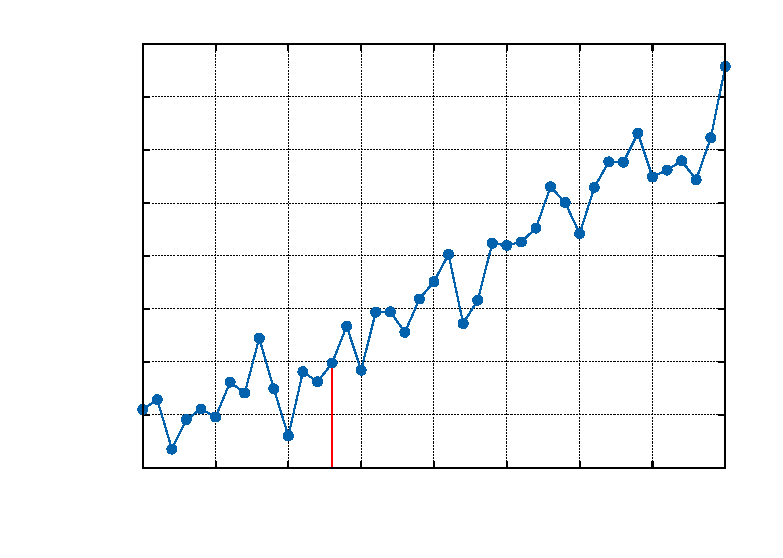
\includegraphics{componentTime}}%
    \gplfronttext
  \end{picture}%
\endgroup
}
	\caption{Running time for different component number}
	\label{fig:component}
	\end{figure}
\end{frame}
% ------------------------------------------
\begin{frame}
	\frametitle{Event Detection Evaluation}
	A event detection task of 16 events. \\ 
	The other six systems are chosen from IEEE AASP Challenge. 
	\begin{figure}[htb!]
	\centering
	\resizebox{0.8\totalheight}{!}{% GNUPLOT: LaTeX picture with Postscript
\begingroup
  \makeatletter
  \providecommand\color[2][]{%
    \GenericError{(gnuplot) \space\space\space\@spaces}{%
      Package color not loaded in conjunction with
      terminal option `colourtext'%
    }{See the gnuplot documentation for explanation.%
    }{Either use 'blacktext' in gnuplot or load the package
      color.sty in LaTeX.}%
    \renewcommand\color[2][]{}%
  }%
  \providecommand\includegraphics[2][]{%
    \GenericError{(gnuplot) \space\space\space\@spaces}{%
      Package graphicx or graphics not loaded%
    }{See the gnuplot documentation for explanation.%
    }{The gnuplot epslatex terminal needs graphicx.sty or graphics.sty.}%
    \renewcommand\includegraphics[2][]{}%
  }%
  \providecommand\rotatebox[2]{#2}%
  \@ifundefined{ifGPcolor}{%
    \newif\ifGPcolor
    \GPcolorfalse
  }{}%
  \@ifundefined{ifGPblacktext}{%
    \newif\ifGPblacktext
    \GPblacktexttrue
  }{}%
  % define a \g@addto@macro without @ in the name:
  \let\gplgaddtomacro\g@addto@macro
  % define empty templates for all commands taking text:
  \gdef\gplbacktext{}%
  \gdef\gplfronttext{}%
  \makeatother
  \ifGPblacktext
    % no textcolor at all
    \def\colorrgb#1{}%
    \def\colorgray#1{}%
  \else
    % gray or color?
    \ifGPcolor
      \def\colorrgb#1{\color[rgb]{#1}}%
      \def\colorgray#1{\color[gray]{#1}}%
      \expandafter\def\csname LTw\endcsname{\color{white}}%
      \expandafter\def\csname LTb\endcsname{\color{black}}%
      \expandafter\def\csname LTa\endcsname{\color{black}}%
      \expandafter\def\csname LT0\endcsname{\color[rgb]{1,0,0}}%
      \expandafter\def\csname LT1\endcsname{\color[rgb]{0,1,0}}%
      \expandafter\def\csname LT2\endcsname{\color[rgb]{0,0,1}}%
      \expandafter\def\csname LT3\endcsname{\color[rgb]{1,0,1}}%
      \expandafter\def\csname LT4\endcsname{\color[rgb]{0,1,1}}%
      \expandafter\def\csname LT5\endcsname{\color[rgb]{1,1,0}}%
      \expandafter\def\csname LT6\endcsname{\color[rgb]{0,0,0}}%
      \expandafter\def\csname LT7\endcsname{\color[rgb]{1,0.3,0}}%
      \expandafter\def\csname LT8\endcsname{\color[rgb]{0.5,0.5,0.5}}%
    \else
      % gray
      \def\colorrgb#1{\color{black}}%
      \def\colorgray#1{\color[gray]{#1}}%
      \expandafter\def\csname LTw\endcsname{\color{white}}%
      \expandafter\def\csname LTb\endcsname{\color{black}}%
      \expandafter\def\csname LTa\endcsname{\color{black}}%
      \expandafter\def\csname LT0\endcsname{\color{black}}%
      \expandafter\def\csname LT1\endcsname{\color{black}}%
      \expandafter\def\csname LT2\endcsname{\color{black}}%
      \expandafter\def\csname LT3\endcsname{\color{black}}%
      \expandafter\def\csname LT4\endcsname{\color{black}}%
      \expandafter\def\csname LT5\endcsname{\color{black}}%
      \expandafter\def\csname LT6\endcsname{\color{black}}%
      \expandafter\def\csname LT7\endcsname{\color{black}}%
      \expandafter\def\csname LT8\endcsname{\color{black}}%
    \fi
  \fi
  \setlength{\unitlength}{0.0500bp}%
  \begin{picture}(7200.00,5040.00)%
    \gplgaddtomacro\gplbacktext{%
      \csname LTb\endcsname%
      \put(1078,440){\makebox(0,0)[r]{\strut{} 0.15}}%
      \csname LTb\endcsname%
      \put(1078,982){\makebox(0,0)[r]{\strut{} 0.2}}%
      \csname LTb\endcsname%
      \put(1078,1524){\makebox(0,0)[r]{\strut{} 0.25}}%
      \csname LTb\endcsname%
      \put(1078,2066){\makebox(0,0)[r]{\strut{} 0.3}}%
      \csname LTb\endcsname%
      \put(1078,2607){\makebox(0,0)[r]{\strut{} 0.35}}%
      \csname LTb\endcsname%
      \put(1078,3149){\makebox(0,0)[r]{\strut{} 0.4}}%
      \csname LTb\endcsname%
      \put(1078,3691){\makebox(0,0)[r]{\strut{} 0.45}}%
      \csname LTb\endcsname%
      \put(1078,4233){\makebox(0,0)[r]{\strut{} 0.5}}%
      \csname LTb\endcsname%
      \put(1078,4775){\makebox(0,0)[r]{\strut{} 0.55}}%
      \csname LTb\endcsname%
      \put(1610,220){\makebox(0,0){\strut{}baseline}}%
      \csname LTb\endcsname%
      \put(2409,220){\makebox(0,0){\strut{}NR2}}%
      \csname LTb\endcsname%
      \put(3208,220){\makebox(0,0){\strut{}NVM}}%
      \csname LTb\endcsname%
      \put(4007,220){\makebox(0,0){\strut{}Our}}%
      \csname LTb\endcsname%
      \put(4806,220){\makebox(0,0){\strut{}VVK}}%
      \csname LTb\endcsname%
      \put(5605,220){\makebox(0,0){\strut{}GVV}}%
      \csname LTb\endcsname%
      \put(6404,220){\makebox(0,0){\strut{}DHV}}%
      \put(176,2607){\rotatebox{-270}{\makebox(0,0){\strut{}Average F-measure}}}%
    }%
    \gplgaddtomacro\gplfronttext{%
    }%
    \gplbacktext
    \put(0,0){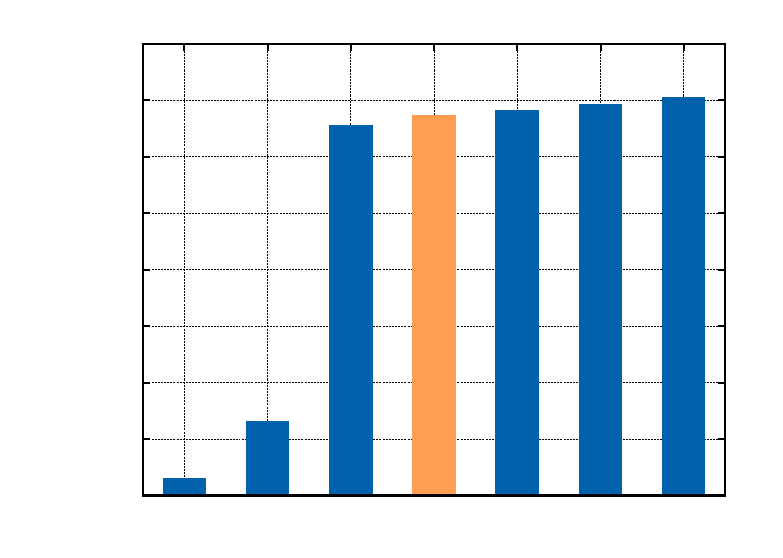
\includegraphics{eventdetectF1}}%
    \gplfronttext
  \end{picture}%
\endgroup
}
	\caption{Event Detection F-Measure}
	\label{fig:eventdetectF1}
	\end{figure}
\end{frame}
% ------------------------------------------
\subsection{Scene Recognition Evaluation}
\begin{frame}
	\frametitle{Scene Recognition Evaluation}
	In scene recognition, we choose 10 scenes, each scene has 10 clips. \\ 	
	Accuracy for other 4 systems are calculated using 5-fold cross validation.
	\begin{figure}[htb!]
	\centering
	\resizebox{0.8\totalheight}{!}{% GNUPLOT: LaTeX picture with Postscript
\begingroup
  \makeatletter
  \providecommand\color[2][]{%
    \GenericError{(gnuplot) \space\space\space\@spaces}{%
      Package color not loaded in conjunction with
      terminal option `colourtext'%
    }{See the gnuplot documentation for explanation.%
    }{Either use 'blacktext' in gnuplot or load the package
      color.sty in LaTeX.}%
    \renewcommand\color[2][]{}%
  }%
  \providecommand\includegraphics[2][]{%
    \GenericError{(gnuplot) \space\space\space\@spaces}{%
      Package graphicx or graphics not loaded%
    }{See the gnuplot documentation for explanation.%
    }{The gnuplot epslatex terminal needs graphicx.sty or graphics.sty.}%
    \renewcommand\includegraphics[2][]{}%
  }%
  \providecommand\rotatebox[2]{#2}%
  \@ifundefined{ifGPcolor}{%
    \newif\ifGPcolor
    \GPcolorfalse
  }{}%
  \@ifundefined{ifGPblacktext}{%
    \newif\ifGPblacktext
    \GPblacktexttrue
  }{}%
  % define a \g@addto@macro without @ in the name:
  \let\gplgaddtomacro\g@addto@macro
  % define empty templates for all commands taking text:
  \gdef\gplbacktext{}%
  \gdef\gplfronttext{}%
  \makeatother
  \ifGPblacktext
    % no textcolor at all
    \def\colorrgb#1{}%
    \def\colorgray#1{}%
  \else
    % gray or color?
    \ifGPcolor
      \def\colorrgb#1{\color[rgb]{#1}}%
      \def\colorgray#1{\color[gray]{#1}}%
      \expandafter\def\csname LTw\endcsname{\color{white}}%
      \expandafter\def\csname LTb\endcsname{\color{black}}%
      \expandafter\def\csname LTa\endcsname{\color{black}}%
      \expandafter\def\csname LT0\endcsname{\color[rgb]{1,0,0}}%
      \expandafter\def\csname LT1\endcsname{\color[rgb]{0,1,0}}%
      \expandafter\def\csname LT2\endcsname{\color[rgb]{0,0,1}}%
      \expandafter\def\csname LT3\endcsname{\color[rgb]{1,0,1}}%
      \expandafter\def\csname LT4\endcsname{\color[rgb]{0,1,1}}%
      \expandafter\def\csname LT5\endcsname{\color[rgb]{1,1,0}}%
      \expandafter\def\csname LT6\endcsname{\color[rgb]{0,0,0}}%
      \expandafter\def\csname LT7\endcsname{\color[rgb]{1,0.3,0}}%
      \expandafter\def\csname LT8\endcsname{\color[rgb]{0.5,0.5,0.5}}%
    \else
      % gray
      \def\colorrgb#1{\color{black}}%
      \def\colorgray#1{\color[gray]{#1}}%
      \expandafter\def\csname LTw\endcsname{\color{white}}%
      \expandafter\def\csname LTb\endcsname{\color{black}}%
      \expandafter\def\csname LTa\endcsname{\color{black}}%
      \expandafter\def\csname LT0\endcsname{\color{black}}%
      \expandafter\def\csname LT1\endcsname{\color{black}}%
      \expandafter\def\csname LT2\endcsname{\color{black}}%
      \expandafter\def\csname LT3\endcsname{\color{black}}%
      \expandafter\def\csname LT4\endcsname{\color{black}}%
      \expandafter\def\csname LT5\endcsname{\color{black}}%
      \expandafter\def\csname LT6\endcsname{\color{black}}%
      \expandafter\def\csname LT7\endcsname{\color{black}}%
      \expandafter\def\csname LT8\endcsname{\color{black}}%
    \fi
  \fi
  \setlength{\unitlength}{0.0500bp}%
  \begin{picture}(7200.00,5040.00)%
    \gplgaddtomacro\gplbacktext{%
      \csname LTb\endcsname%
      \put(946,440){\makebox(0,0)[r]{\strut{} 0}}%
      \csname LTb\endcsname%
      \put(946,1059){\makebox(0,0)[r]{\strut{} 0.1}}%
      \csname LTb\endcsname%
      \put(946,1679){\makebox(0,0)[r]{\strut{} 0.2}}%
      \csname LTb\endcsname%
      \put(946,2298){\makebox(0,0)[r]{\strut{} 0.3}}%
      \csname LTb\endcsname%
      \put(946,2917){\makebox(0,0)[r]{\strut{} 0.4}}%
      \csname LTb\endcsname%
      \put(946,3536){\makebox(0,0)[r]{\strut{} 0.5}}%
      \csname LTb\endcsname%
      \put(946,4156){\makebox(0,0)[r]{\strut{} 0.6}}%
      \csname LTb\endcsname%
      \put(946,4775){\makebox(0,0)[r]{\strut{} 0.7}}%
      \csname LTb\endcsname%
      \put(1681,220){\makebox(0,0){\strut{}Baseline}}%
      \csname LTb\endcsname%
      \put(2886,220){\makebox(0,0){\strut{}RNH1}}%
      \csname LTb\endcsname%
      \put(4091,220){\makebox(0,0){\strut{}RNH2}}%
      \csname LTb\endcsname%
      \put(5296,220){\makebox(0,0){\strut{}Our}}%
      \csname LTb\endcsname%
      \put(6502,220){\makebox(0,0){\strut{}GSR}}%
      \put(176,2607){\rotatebox{-270}{\makebox(0,0){\strut{}\LARGE{Average Accuracy}}}}%
    }%
    \gplgaddtomacro\gplfronttext{%
    }%
    \gplbacktext
    \put(0,0){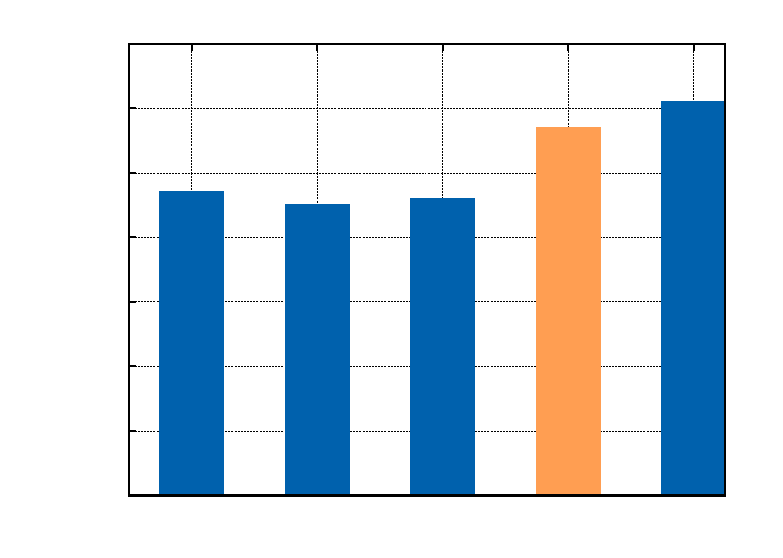
\includegraphics{sceneeval}}%
    \gplfronttext
  \end{picture}%
\endgroup
}
	\caption{Recognition accuracy for 10 audio scenes}
	\label{fig:sceneeval}
	\end{figure}
\end{frame}
% ------------------------------------------
\begin{frame}
	\frametitle{Scene Recognition Evaluation}
	Detailed result of our system with the best system \textit{GSR}. \\ 
	\begin{figure}[htb!]
	\centering
	\resizebox{0.8\totalheight}{!}{% GNUPLOT: LaTeX picture with Postscript
\begingroup
  \makeatletter
  \providecommand\color[2][]{%
    \GenericError{(gnuplot) \space\space\space\@spaces}{%
      Package color not loaded in conjunction with
      terminal option `colourtext'%
    }{See the gnuplot documentation for explanation.%
    }{Either use 'blacktext' in gnuplot or load the package
      color.sty in LaTeX.}%
    \renewcommand\color[2][]{}%
  }%
  \providecommand\includegraphics[2][]{%
    \GenericError{(gnuplot) \space\space\space\@spaces}{%
      Package graphicx or graphics not loaded%
    }{See the gnuplot documentation for explanation.%
    }{The gnuplot epslatex terminal needs graphicx.sty or graphics.sty.}%
    \renewcommand\includegraphics[2][]{}%
  }%
  \providecommand\rotatebox[2]{#2}%
  \@ifundefined{ifGPcolor}{%
    \newif\ifGPcolor
    \GPcolorfalse
  }{}%
  \@ifundefined{ifGPblacktext}{%
    \newif\ifGPblacktext
    \GPblacktexttrue
  }{}%
  % define a \g@addto@macro without @ in the name:
  \let\gplgaddtomacro\g@addto@macro
  % define empty templates for all commands taking text:
  \gdef\gplbacktext{}%
  \gdef\gplfronttext{}%
  \makeatother
  \ifGPblacktext
    % no textcolor at all
    \def\colorrgb#1{}%
    \def\colorgray#1{}%
  \else
    % gray or color?
    \ifGPcolor
      \def\colorrgb#1{\color[rgb]{#1}}%
      \def\colorgray#1{\color[gray]{#1}}%
      \expandafter\def\csname LTw\endcsname{\color{white}}%
      \expandafter\def\csname LTb\endcsname{\color{black}}%
      \expandafter\def\csname LTa\endcsname{\color{black}}%
      \expandafter\def\csname LT0\endcsname{\color[rgb]{1,0,0}}%
      \expandafter\def\csname LT1\endcsname{\color[rgb]{0,1,0}}%
      \expandafter\def\csname LT2\endcsname{\color[rgb]{0,0,1}}%
      \expandafter\def\csname LT3\endcsname{\color[rgb]{1,0,1}}%
      \expandafter\def\csname LT4\endcsname{\color[rgb]{0,1,1}}%
      \expandafter\def\csname LT5\endcsname{\color[rgb]{1,1,0}}%
      \expandafter\def\csname LT6\endcsname{\color[rgb]{0,0,0}}%
      \expandafter\def\csname LT7\endcsname{\color[rgb]{1,0.3,0}}%
      \expandafter\def\csname LT8\endcsname{\color[rgb]{0.5,0.5,0.5}}%
    \else
      % gray
      \def\colorrgb#1{\color{black}}%
      \def\colorgray#1{\color[gray]{#1}}%
      \expandafter\def\csname LTw\endcsname{\color{white}}%
      \expandafter\def\csname LTb\endcsname{\color{black}}%
      \expandafter\def\csname LTa\endcsname{\color{black}}%
      \expandafter\def\csname LT0\endcsname{\color{black}}%
      \expandafter\def\csname LT1\endcsname{\color{black}}%
      \expandafter\def\csname LT2\endcsname{\color{black}}%
      \expandafter\def\csname LT3\endcsname{\color{black}}%
      \expandafter\def\csname LT4\endcsname{\color{black}}%
      \expandafter\def\csname LT5\endcsname{\color{black}}%
      \expandafter\def\csname LT6\endcsname{\color{black}}%
      \expandafter\def\csname LT7\endcsname{\color{black}}%
      \expandafter\def\csname LT8\endcsname{\color{black}}%
    \fi
  \fi
  \setlength{\unitlength}{0.0500bp}%
  \begin{picture}(7200.00,5040.00)%
    \gplgaddtomacro\gplbacktext{%
      \csname LTb\endcsname%
      \put(946,440){\makebox(0,0)[r]{\strut{} 0}}%
      \csname LTb\endcsname%
      \put(946,1163){\makebox(0,0)[r]{\strut{} 0.2}}%
      \csname LTb\endcsname%
      \put(946,1885){\makebox(0,0)[r]{\strut{} 0.4}}%
      \csname LTb\endcsname%
      \put(946,2608){\makebox(0,0)[r]{\strut{} 0.6}}%
      \csname LTb\endcsname%
      \put(946,3330){\makebox(0,0)[r]{\strut{} 0.8}}%
      \csname LTb\endcsname%
      \put(946,4053){\makebox(0,0)[r]{\strut{} 1}}%
      \csname LTb\endcsname%
      \put(946,4775){\makebox(0,0)[r]{\strut{} 1.2}}%
      \csname LTb\endcsname%
      \put(1374,88){\rotatebox{45}{\makebox(0,0){\strut{}bathroom}}}%
      \csname LTb\endcsname%
      \put(1966,88){\rotatebox{45}{\makebox(0,0){\strut{}beach}}}%
      \csname LTb\endcsname%
      \put(2559,88){\rotatebox{45}{\makebox(0,0){\strut{}concert}}}%
      \csname LTb\endcsname%
      \put(3151,88){\rotatebox{45}{\makebox(0,0){\strut{}forest}}}%
      \csname LTb\endcsname%
      \put(3743,88){\rotatebox{45}{\makebox(0,0){\strut{}kitchen}}}%
      \csname LTb\endcsname%
      \put(4335,88){\rotatebox{45}{\makebox(0,0){\strut{}office}}}%
      \csname LTb\endcsname%
      \put(4928,88){\rotatebox{45}{\makebox(0,0){\strut{}park}}}%
      \csname LTb\endcsname%
      \put(5520,88){\rotatebox{45}{\makebox(0,0){\strut{}restaurant}}}%
      \csname LTb\endcsname%
      \put(6112,88){\rotatebox{45}{\makebox(0,0){\strut{}street}}}%
      \csname LTb\endcsname%
      \put(6704,88){\rotatebox{45}{\makebox(0,0){\strut{}subway station}}}%
      \put(176,2607){\rotatebox{-270}{\makebox(0,0){\strut{}Scene Recognition Accuracy (Our vs. GSR)}}}%
    }%
    \gplgaddtomacro\gplfronttext{%
      \csname LTb\endcsname%
      \put(5816,4602){\makebox(0,0)[r]{\strut{}GSR}}%
      \csname LTb\endcsname%
      \put(5816,4382){\makebox(0,0)[r]{\strut{}Our}}%
    }%
    \gplbacktext
    \put(0,0){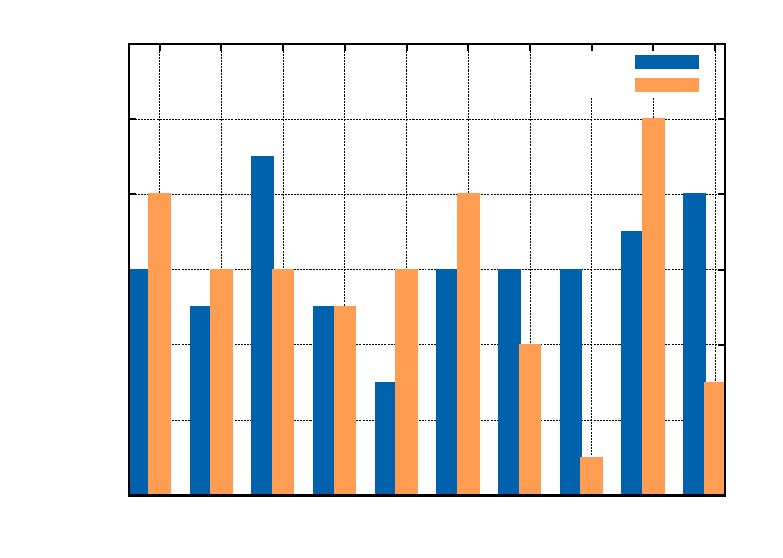
\includegraphics{ourgsr}}%
    \gplfronttext
  \end{picture}%
\endgroup
}
	\caption{10 scenes comparison}
	\label{fig:sceneeval}
	\end{figure}
\end{frame}
% ------------------------------------------
\section{Demo}
\begin{frame}
	\frametitle{Demo}
	Live demo for our system. 
\end{frame}
% ------------------------------------------
\begin{frame}
	\frametitle{Acknowledgement}
	I would like to thank my advisor Kenny Q. Zhu, and my friend Xinyu Hua for their help in this project. 
\end{frame}
% ------------------------------------------
%\setbeamertemplate{background canvas}[vertical shading][bottom=white,top=structure.fg!25]
\begin{frame}
  \begin{center}
    {\huge \emph{{Thank  ~you!
          \\   \vspace{1cm} Any Question?}}}
  \end{center}
\end{frame}
\end{document}
